\chapter{Experiments}\label{chap:experiments}

Experiments often include benchmarks.
You need to describe you benchmarking setup: parameters of the machine used (architecture, memory, etc), parameters of the software used (OS version, libraries used and their version), the benchmark programs.
The programs need not be part of the thesis, but they should be described and available separately.

If you measure run times and evaluate your findings statistically, then there is great potential for errors.
Consult SIGPLAN's checklist for empirical evaluations \url{http://www.sigplan.org/Resources/EmpiricalEvaluation/} for advice. 

\definecolor{myellow}{RGB}{228,212,0}
\definecolor{mgreen}{RGB}{5,104,57}

\newcommand\funnel[3]{%
\pgfmathsetmacro\mwid{(0.3+\val*0.06)}
\pgfmathsetmacro\mradius{(\val*0.01 + 1)}
\pgfmathsetmacro\mheight{(\val*0.003 + 0.4)}
\pgfmathsetmacro\marc{\mwid-.4}
    \begin{scope}[%
        shift={(0,#1)}, 
        line width=.05pt, 
        %x=5mm, 
        %scale=1.\xi,
        yshift=\xi*4
        ]
    \draw[black,bottom color=#2, top color=#2] (-\mwid,0) -- (-\mwid+.4,-\mheight) arc (190:350:\marc cm and \mradius mm) -- (\mwid,0);
    \draw[black,fill=#3] (0,0) ellipse (\mwid cm and \mradius mm);
    \path (-\mwid,0) -- (-\mwid+.4,-\mheight) coordinate[midway] (a\xi);
    \end{scope}
}

\begin{figure}[h]
	\hspace*{-0.28\textwidth}
	\centering
	\begin{tikzpicture}
		\foreach \val
				[%
				count=\xi starting from 0, 
				evaluate=\xi as \shadecolor using int(25*\xi),
				evaluate=\xi as \coord using int(\xi-12)
				]
			in {
				4.05,
				9.37,
				24.02,
				37.49,
				71.19,
				82.50,
				100.00
			}{
				\funnel{\coord}{mgreen!\shadecolor !myellow}{mgreen!\shadecolor !myellow}
			}   

		\node[left=0.02\textwidth of a0] {Generated Declaration Files};
		\node[right=0.07\textwidth of a0] {\textbf{244}};

		\node[left=0.02\textwidth of a1] {Run-time Information};
		\node[right=0.12\textwidth of a1] {\textbf{565}};

		\node[left=0.02\textwidth of a2] {Working Examples};
		\node[right=0.26\textwidth of a2] {\textbf{1448}};

		\node[left=0.02\textwidth of a3] {Code Examples};
		\node[right=0.38\textwidth of a3] {\textbf{2260}};

		\node[left=0.02\textwidth of a4] {README file};
		\node[right=0.70\textwidth of a4] {\textbf{4292}};

		\node[left=0.02\textwidth of a5] {Github Repository};
		\node[right=0.80\textwidth of a5] {\textbf{4974}};

		\node[align=right,left=0.02\textwidth of a6, text width=0.25\textwidth] {Definitely Typed Modules};
		\node[right=0.97\textwidth of a6] {\textbf{6029}};

	\end{tikzpicture}
	\caption[Number of analyzed modules for each stage of the experiment]{\textbf{Number of analyzed modules for each stage of the experiment} - A TypeScript Declaration File was generated for only 244 modules, out of 6029 modules in the DefinitelyTyped Repository. It was possible to gather valid run-time information for only 25\% of the modules for which a Code Example was extracted.}
\end{figure}


\section{Definitely Typed Modules}
\section{Code Examples Extraction}
\subsection{Repositories URL}
\subsection{Readme Files}
\subsection{Code Examples}

\section{Code Execution}

\section{Run-time Information Gathering}

\section{Declaration Files Generation}

\section{Evaluation}

\section{JS Operators Usage}
\todo{Agregar que es una matriz simetrica. Que era para hacer un analisis mas global. Para algunos operators se puede inferir que el orden de los tipos sí afecta. Por ejemplo para instance of donde obviamente importa el orden. Pero para == por ejemplo generalmente se pone a == null y no null == a}.
\begin{figure}[tp]
	\centering

	\begin{tikzpicture}
		\begin{axis}[
			view={0}{90},
			title=Operator ${<}$,
			width=0.45\textwidth,
			colormap/hot,
			xticklabels={number,string,undefined,object,null,boolean,function,array},
			xtick={0,...,7},
			yticklabels={number,string,undefined,object,null,boolean,function,array},
			ytick={7,...,0},
			x tick label style={rotate=90,anchor=east}]
		]
		\addplot3[surf, shader=interp, left] file {figures/experiments/operators/relational-operators/operator_<.dat};
		\end{axis}
	\end{tikzpicture}
	%
	\begin{tikzpicture}
		\begin{axis}[
			view={0}{90},
			width=0.45\textwidth,
			title=Operator ${>}$,
			colormap/hot,
			xticklabels={number,string,undefined,object,null,boolean,function,array},
			xtick={0,...,7},
			yticklabels={number,string,undefined,object,null,boolean,function,array},
			ytick={7,...,0},
			x tick label style={rotate=90,anchor=east}]
		\addplot3[surf, shader=interp, left] file {figures/experiments/operators/relational-operators/operator_>.dat};
		\end{axis}
	\end{tikzpicture}

	\centering
	\begin{tikzpicture}
		\begin{axis}[
			view={0}{90},
			width=0.45\textwidth,
			title=Operator ${<=}$,
			colormap/hot,
			xticklabels={number,string,undefined,object,null,boolean,function,array},
			xtick={0,...,7},
			yticklabels={number,string,undefined,object,null,boolean,function,array},
			ytick={7,...,0},
			x tick label style={rotate=90,anchor=east}]
		\addplot3[surf, shader=interp, left] file {figures/experiments/operators/relational-operators/operator_<=.dat};
		\end{axis}
	\end{tikzpicture}
	%
	\begin{tikzpicture}
		\begin{axis}[
			view={0}{90},
			width=0.45\textwidth,
			title=Operator ${>=}$,
			colormap/hot,
			xticklabels={number,string,undefined,object,null,boolean,function,array},
			xtick={0,...,7},
			yticklabels={number,string,undefined,object,null,boolean,function,array},
			ytick={7,...,0},
			x tick label style={rotate=90,anchor=east}]
		\addplot3[surf, shader=interp, left] file {figures/experiments/operators/relational-operators/operator_>=.dat};
		\end{axis}
	\end{tikzpicture}
	
	\centering
	\begin{tikzpicture}
		\begin{axis}[
			view={0}{90},
			width=0.45\textwidth,
			title=Operator ${instanceof}$,
			colormap/hot,
			xticklabels={number,string,undefined,object,null,boolean,function,array},
			xtick={0,...,7},
			yticklabels={number,string,undefined,object,null,boolean,function,array},
			ytick={7,...,0},
			x tick label style={rotate=90,anchor=east}]
		\addplot3[surf, shader=interp, left] file {figures/experiments/operators/relational-operators/operator_instanceof.dat};
		\end{axis}
	\end{tikzpicture}
	%
	\begin{tikzpicture}
		\begin{axis}[
			view={0}{90},
			width=0.45\textwidth,
			title=Operator ${in}$,
			colormap/hot,
			xticklabels={number,string,undefined,object,null,boolean,function,array},
			xtick={0,...,7},
			yticklabels={number,string,undefined,object,null,boolean,function,array},
			ytick={7,...,0},
			x tick label style={rotate=90,anchor=east}]
		\addplot3[surf, shader=interp, left] file {figures/experiments/operators/relational-operators/operator_in.dat};
		\end{axis}
	\end{tikzpicture}

	\centering
	\hspace{0.1\textwidth}
	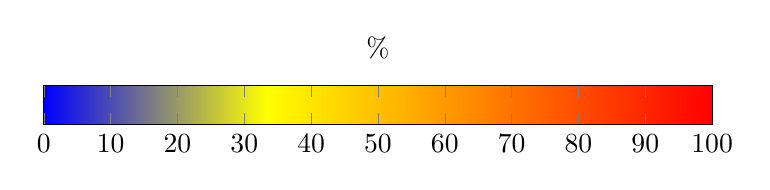
\begin{tikzpicture}
		\begin{axis}[
			hide axis,
			scale only axis,
			height=0pt,
			width=0pt,
			colormap/hot,
			colorbar horizontal,
			point meta min=0,
			point meta max=100,
			colorbar style={
				title=\%,
				width=0.7\textwidth,
				xtick={0, 10, 20, 30, 40, ..., 100}
			}]
			\addplot [draw=none] coordinates {(0,0)};
		\end{axis}
	\end{tikzpicture}
	\caption[Relational operators]{\textbf{Type distribution for relational operators} - Operators ${<}$, ${>}$, ${<=}$, ${>=}$ are mainly used with the \textit{number-number} combination}
	\label{fig:experiments-relational-operators}
\end{figure}
\begin{figure}[tp]
	\centering

	\begin{tikzpicture}
		\begin{axis}[
			view={0}{90},
			title=Operator ${+}$,
			width=0.45\textwidth,
			colormap/hot,
			xticklabels={number,string,undefined,object,null,boolean,function,array},
			xtick={0,...,7},
			yticklabels={number,string,undefined,object,null,boolean,function,array},
			ytick={7,...,0},
			x tick label style={rotate=90,anchor=east}]
		]
		\addplot3[surf, shader=interp, left] file {figures/experiments/operators/additive-operators/operator_+.dat};
		\end{axis}
	\end{tikzpicture}
	%
	\begin{tikzpicture}
		\begin{axis}[
			view={0}{90},
			width=0.45\textwidth,
			title=Operator ${-}$,
			colormap/hot,
			xticklabels={number,string,undefined,object,null,boolean,function,array},
			xtick={0,...,7},
			yticklabels={number,string,undefined,object,null,boolean,function,array},
			ytick={7,...,0},
			x tick label style={rotate=90,anchor=east}]
		\addplot3[surf, shader=interp, left] file {figures/experiments/operators/additive-operators/operator_-.dat};
		\end{axis}
	\end{tikzpicture}

	\centering
	\hspace{0.1\textwidth}
	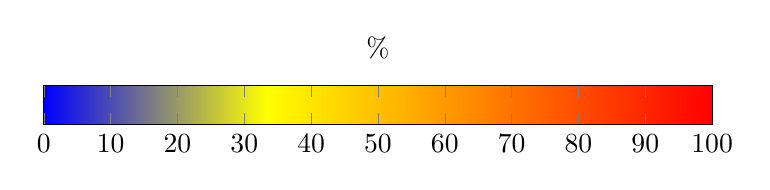
\begin{tikzpicture}
		\begin{axis}[
			hide axis,
			scale only axis,
			height=0pt,
			width=0pt,
			colormap/hot,
			colorbar horizontal,
			point meta min=0,
			point meta max=100,
			colorbar style={
				title=\%,
				width=0.7\textwidth,
				xtick={0, 10, 20, 30, 40, ..., 100}
			}]
			\addplot [draw=none] coordinates {(0,0)};
		\end{axis}
	\end{tikzpicture}
	\caption[Additive operators]{\textbf{Type distribution for additive operators} - Both operators are mainly used with the \textit{number-number} combination. Operator $+$ is also used for pure string concatenation. However, due to JS Type Coercion, $+$ is also used for \textit{string} and \textit{number} concatenation}
	\label{fig:experiments-additive-operators}
\end{figure}
\begin{figure}[h]
	\centering

	\begin{tikzpicture}
		\begin{axis}[
			view={0}{90},
			title=Operator ${*}$,
			width=0.45\textwidth,
			colormap/hot,
			xticklabels={number,string,undefined,object,null,boolean,function,array},
			xtick={0,...,7},
			yticklabels={number,string,undefined,object,null,boolean,function,array},
			ytick={7,...,0},
			x tick label style={rotate=90,anchor=east}]
		]
		\addplot3[surf, shader=interp, left] file {figures/experiments/operators/multiplicative-operators/operator_star.dat};
		\end{axis}
	\end{tikzpicture}
	%
	\begin{tikzpicture}
		\begin{axis}[
			view={0}{90},
			width=0.45\textwidth,
			title=Operator ${/}$,
			colormap/hot,
			xticklabels={number,string,undefined,object,null,boolean,function,array},
			xtick={0,...,7},
			yticklabels={number,string,undefined,object,null,boolean,function,array},
			ytick={7,...,0},
			x tick label style={rotate=90,anchor=east}]
		\addplot3[surf, shader=interp, left] file {figures/experiments/operators/multiplicative-operators/operator_division.dat};
		\end{axis}
	\end{tikzpicture}

	\centering
	\begin{tikzpicture}
		\begin{axis}[
			view={0}{90},
			width=0.45\textwidth,
			title=Operator ${\%}$,
			colormap/hot,
			xticklabels={number,string,undefined,object,null,boolean,function,array},
			xtick={0,...,7},
			yticklabels={number,string,undefined,object,null,boolean,function,array},
			ytick={7,...,0},
			x tick label style={rotate=90,anchor=east}]
		\addplot3[surf, shader=interp, left] file {figures/experiments/operators/multiplicative-operators/operator_percentage.dat};
		\end{axis}
	\end{tikzpicture}
	
	\centering
	\hspace{0.1\textwidth}
	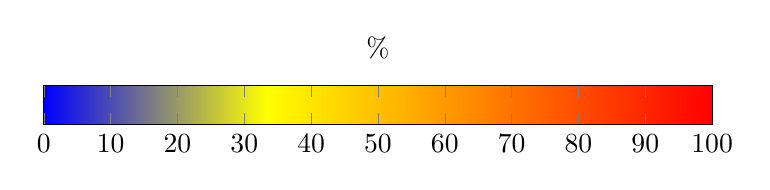
\begin{tikzpicture}
		\begin{axis}[
			hide axis,
			scale only axis,
			height=0pt,
			width=0pt,
			colormap/hot,
			colorbar horizontal,
			point meta min=0,
			point meta max=100,
			colorbar style={
				title=\%,
				width=0.7\textwidth,
				xtick={0, 10, 20, 30, 40, ..., 100}
			}]
			\addplot [draw=none] coordinates {(0,0)};
		\end{axis}
	\end{tikzpicture}
	\caption[Relational operators]{\textbf{Type distribution for multiplicative operators} - All multiplicative operators are mainly used with the \textit{number-number} combination}
\end{figure}
\begin{figure}[h]
	\centering

	\begin{tikzpicture}
		\begin{axis}[
			view={0}{90},
			title=Operator ${==}$,
			width=0.45\textwidth,
			colormap/hot,
			xticklabels={number,string,undefined,object,null,boolean,function,array},
			xtick={0,...,7},
			yticklabels={number,string,undefined,object,null,boolean,function,array},
			ytick={7,...,0},
			x tick label style={rotate=90,anchor=east}]
		]
		\addplot3[surf, shader=interp, left] file {figures/experiments/operators/equality-operators/operator_==.dat};
		\end{axis}
	\end{tikzpicture}
	%
	\begin{tikzpicture}
		\begin{axis}[
			view={0}{90},
			width=0.45\textwidth,
			title=Operator ${!=}$,
			colormap/hot,
			xticklabels={number,string,undefined,object,null,boolean,function,array},
			xtick={0,...,7},
			yticklabels={number,string,undefined,object,null,boolean,function,array},
			ytick={7,...,0},
			x tick label style={rotate=90,anchor=east}]
		\addplot3[surf, shader=interp, left] file {figures/experiments/operators/equality-operators/operator_!=.dat};
		\end{axis}
	\end{tikzpicture}

	\centering
	\begin{tikzpicture}
		\begin{axis}[
			view={0}{90},
			width=0.45\textwidth,
			title=Operator ${===}$,
			colormap/hot,
			xticklabels={number,string,undefined,object,null,boolean,function,array},
			xtick={0,...,7},
			yticklabels={number,string,undefined,object,null,boolean,function,array},
			ytick={7,...,0},
			x tick label style={rotate=90,anchor=east}]
		\addplot3[surf, shader=interp, left] file {figures/experiments/operators/equality-operators/operator_===.dat};
		\end{axis}
	\end{tikzpicture}
	%
	\begin{tikzpicture}
		\begin{axis}[
			view={0}{90},
			width=0.45\textwidth,
			title=Operator ${!==}$,
			colormap/hot,
			xticklabels={number,string,undefined,object,null,boolean,function,array},
			xtick={0,...,7},
			yticklabels={number,string,undefined,object,null,boolean,function,array},
			ytick={7,...,0},
			x tick label style={rotate=90,anchor=east}]
		\addplot3[surf, shader=interp, left] file {figures/experiments/operators/equality-operators/operator_!==.dat};
		\end{axis}
	\end{tikzpicture}

	\centering
	\hspace{0.1\textwidth}
	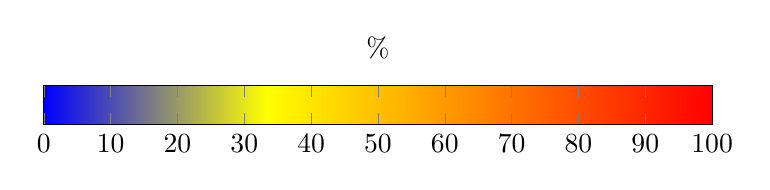
\begin{tikzpicture}
		\begin{axis}[
			hide axis,
			scale only axis,
			height=0pt,
			width=0pt,
			colormap/hot,
			colorbar horizontal,
			point meta min=0,
			point meta max=100,
			colorbar style={
				title=\%,
				width=0.7\textwidth,
				xtick={0, 10, 20, 30, 40, ..., 100}
			}]
			\addplot [draw=none] coordinates {(0,0)};
		\end{axis}
	\end{tikzpicture}
	\caption[Relational operators]{
		\textbf{Type distribution for equality operators} - Operator ${==}$ is mainly used for number comparison. String comparison is performed by using ${===}$ and ${!==}$ operators. Comparison against \textit{null} is performed by using both ${!=}$ and ${!==}$ operators
	}
\end{figure}
\begin{figure}[tp]
	\centering
	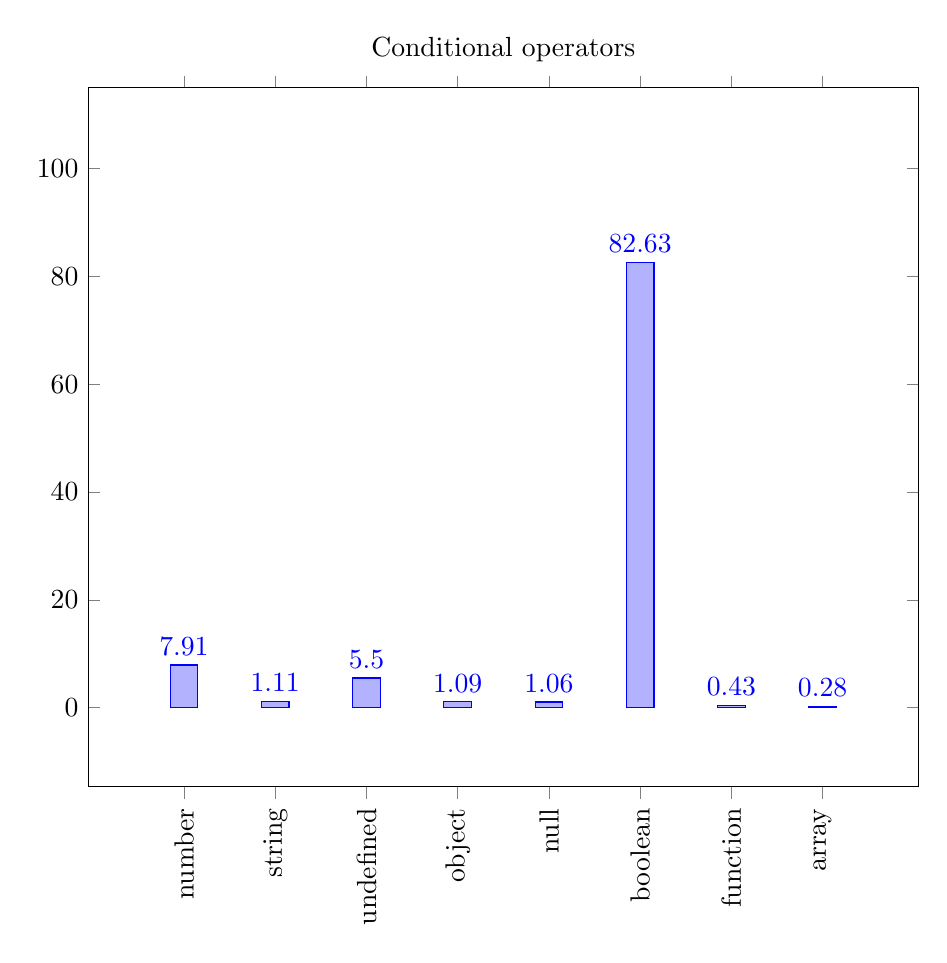
\begin{tikzpicture}
		\begin{axis}[
			ybar,
			title=Conditional operators,
			width=1\textwidth,
			ybar=0pt,
			ymax=100,
			enlargelimits=0.15,
			legend style={at={(0.5,-0.2)}, anchor=north,legend columns=-1},
			symbolic x coords={number,string,undefined,object,null,boolean,function,array},
			xtick=data,
			nodes near coords, 
			nodes near coords align={vertical},
			x tick label style={rotate=90,anchor=east},
		]
		\addplot coordinates {
			(number, 7.91)
			(string, 1.11)
			(undefined, 5.50)
			(object, 1.09)
			(null, 1.06)
			(boolean, 82.63)
			(function, 0.43)
			(array, 0.28)
		};
		\end{axis}
	\end{tikzpicture}
	\caption[Conditional operators]{\textbf{Type distribution for conditional operators} - It includes all operators that trigger a condition check before branching: ${if-then-else}$, ${switch-case}$, ${while}$, ${for}$, ${||}$, ${\&\&}$, ${ ? : }$.
	}
\end{figure}